\documentclass[12pt]{article}
\usepackage[paperwidth=8.5in,paperheight=11in,margin=1in]{geometry}
\usepackage{float}
\usepackage{lipsum}
\usepackage{parskip}
\usepackage{bbding}
\usepackage{amssymb}
\usepackage{titlesec} 
\usepackage{graphicx}
\usepackage{hyperref}
\usepackage{setspace}
\usepackage[normalem]{ulem}
\usepackage[section]{placeins}
\usepackage[toc,page]{appendix}
\newcounter{subsubsubsection}[subsubsection]
\newcommand{\tline}{\hspace{-2.3pt}$\bullet$ \hspace{5pt}}
\hypersetup{colorlinks=true, linkcolor=black, urlcolor=blue}
\setlength{\parindent}{15pt} % Indent paragraphs (automatically)
\usepackage{pdfpages}

\makeatother
\makeatletter
\setlength{\@fptop}{0pt}

\begin{document}
	\begin{titlepage}
		\centering	
%		\vspace{.25cm}
    
    \begin{figure}[h]
      \centering
%      \includegraphics[width=0.45\linewidth]{icon for team goes here}
    \end{figure} 
  
  {\huge\bfseries LEaD Design: \\ Team Portfolio\par}
    
    \vspace{2cm}
    
		{ \setstretch{0.1}		
  		{\Large\itshape Adrian Beehner\par}
  		{\Large\itshape Andrew Butler\par}
  		{\Large\itshape Paul Martin\par}
  		{\Large\itshape Kevin Dorscher\par}	
		}		
    
    \vspace{2cm} 
    
    {\scshape\Large 
      CS 480/481: Fall 2017 - Spring 2018 \\
      Senior Capstone Design Project \\ 
      UI CS - Wireless Tower of Lights
      \par}
    
     \vspace{7cm} 
    
    \begin{figure}[h]
      \centering
      
\includegraphics[width=0.7\linewidth]{uislogan}
    \end{figure} 
  
		\vfill		
	\end{titlepage}

	\tableofcontents
	\newpage
	
	\section{Introduction}
	
		\subsection{Project Summary}
		The University of Idaho has, for several years, done various projects involving the Tower of Lights Show and equipping the marching band with light-up glasses. The current "TowerLights" product involves LED-based light bars that are placed in front of front-facing widows of a large buildling (Theophilus Tower) and are then illuminated to play animations alongside/synchronously with music. The goal is to enhance the current "TowerLights" product. The current implementation of this product uses the ethernet wiring system in the building to control the LEDs. The goal of the project described in this document is to convert this part of the system to a wireless operation. This in turn requires the development of a wireless module that would be attached to each of the light bars. Thus this module has to sleep and wake up, as well as respond to wireless signals from a computer, and since it's wireless, these modules will need to be battery powered. Battery power must also be conserved by staying in the sleep state until needed. The purpose of this enhancement is to provide a certain level of portability to have "TowerLights" at other locations. \\
		The product will give the user the ability to run a program that reads in .tan files and .wav files, have this program communicate with a XBee Wireless module on an Arduino that is attached to a computer via USB, then communicate wirelessly with each Arduino receiver, that is battery powered. Each of these Arduino receivers are attached to an LED board, that will then communicate with each LED on that board through wired communication from the Arduino (same one that holds the receiver) to the LEDs. The program that broadcasts the shows will be available for OSX, Windows, and Linux based operating systems.\\
		This documentation lives at \url{https://github.com/YupHio/LEaD_Design/tree/master/Doc/TeamPortfolio_LEaD_Design.tex} \\
		The code for the project can be found at \url{https://github.com/YupHio/LEaD_Design/tree/master/Code}
		
		\subsection{Document Purpose}
	 		This document is a team portfolio for the Fall 2017-Spring 2018 CS 480/481: Senior Capstone Design project at the University of Idaho. The purpose of this document is to outline the methodology, design, and keep a record of this project. It defines terms used, outlines the scope of the project, details specific design choices, meeting minutes, project learning, design goals, specification and constraints, system diagrams, analysis of alternatives, engineering modeling, manufacturing/assembly plan, experimental design, data analysis, balance sheet, and other items.
		
		\subsection{Definition of Terms}
			\begin{itemize}
				\item \textbf{Arduino} - open source computer hardware and software company, project, and user community that designs and manufactures 		single-board microcontrollers and microcontroller kits for building digital devices and interactive objects that can sense and control objects in the physical world\\ (https://en.wikipedia.org/wiki/Arduino)
				\item \textbf{Arduino Shield} - Shields are boards that can be plugged on top of the Arduino PCB extending its capabilities. The different shields follow the same philosophy as the original toolkit: they are easy to mount, and cheap to produce.\\ (https://www.arduino.cc/en/Main/ArduinoShields)
				\item \textbf{Xbee} - The Arduino Xbee shield allows multiple Arduino boards to communicate wirelessly over distances up to 100 feet (indoors) or 300 feet (outdoors) using the Maxstream Xbee Zigbee module.\\ (https://www.arduino.cc/en/Main/ArduinoShields)		
			\end{itemize}
		
		\subsubsection{Arduino IDE}
		The Arduino Integrated Development Environment - or Arduino Software (IDE) - contains a text editor for writing code, a message area, a text console, a toolbar with buttons for common functions and a series of menus. It connects to the Arduino and Genuino hardware to upload programs and communicate with them. \url{https://www.arduino.cc/en/Main/Software}
		
		\subsubsection{Pulse}
		 PulseAudio is a sound system for POSIX OSes, meaning that it is a proxy for your sound applications. It allows you to do advanced operations on your sound data as it passes between your application and your hardware. Things like transferring the audio to a different machine, changing the sample format or channel count and mixing several sounds into one are easily achieved using a sound server. \url{https://www.freedesktop.org/wiki/Software/PulseAudio/l}
		
	\newpage

\section{Meeting Minutes}
	Weekly action items and summaries of progress made are detailed below. Furthermore, subsections discuss what was helpful and what was not during these meetings. Discussion of attendance and participation, as well as contribution and discussion topics are discussed below.
	
	\subsubsection{9/08/2017 Meeting Notes - With Dr.Rinker}

	Meeting started at 3:31, all members present, Adrian on Zoom meeting

Question and Answer with Rinker:

General schedule: Rinker's in CDA start of the week, always in Moscow on Friday, in between depends on events.

Current system in the tower: 3 high powered LEDs (in series) in each room facing the proper direction, controlled over CAT cable from the basement. LEDs prefer constant current over constant voltage, using constant current power source. Each color takes 270 mili-amps. Constant current circuit used here.

Future objectives: Convert system to be wireless. Nodes will need to sleep for a couple days before the show begins, using low power, and should then be remotely wake-able. Power and LED configurations are up to us.

Current goofy lights: broadcast from laptop to Arduino like board, transmits out to the glasses. Wireless protocol related to Zigby. Not wifi, but 802.15.4 (ad-hoc sensor network). Devices can sleep, wakeup, reconnect to network, etc. Zigby handles errors when reconnecting, etc. We avoid using Zigby as we’re broadcasting in real time, and do not want the error handling. Broadcasts on 2.4ghz, regular wifi frequency. 9v lith-ion batteries are being used in the glasses. LEDs in the glasses are in series. Uses a resistor to deliver the correct voltage. Uses the chip from an Arduino, straight up programmed from the Arduino IDE. Atmega328p. Broadcasts to all glasses i.e. DMX. Uses 16 different channels for groups of lights.

802.15.4 only goes at 250kbps. Might want to reduce each channel to 2 bytes instead of 3?

DMX protocol: Used in theater lights, wired protocol, goes through each light sequentially.

Current code is all available for use, we're going to get that from Rinker and put on GitHub(?)

Mouser.com parts. Superbrightleds.com	

Meeting adjourned at 4:39
	
	\subsubsection{9/14/2017 Meeting Notes}
	Meeting started at 3:30, Adrian lost Internet almost immediately (bad ISP). This Team meeting had the team generally discuss the schedule of the project for the entire year. This meeting was very important in outlining the goals and deadlines needed on a monthly basis. The figures for these schedules is shown below. Meeting ended at 4:15
	
	\begin{figure}[!htb]
		\centering
		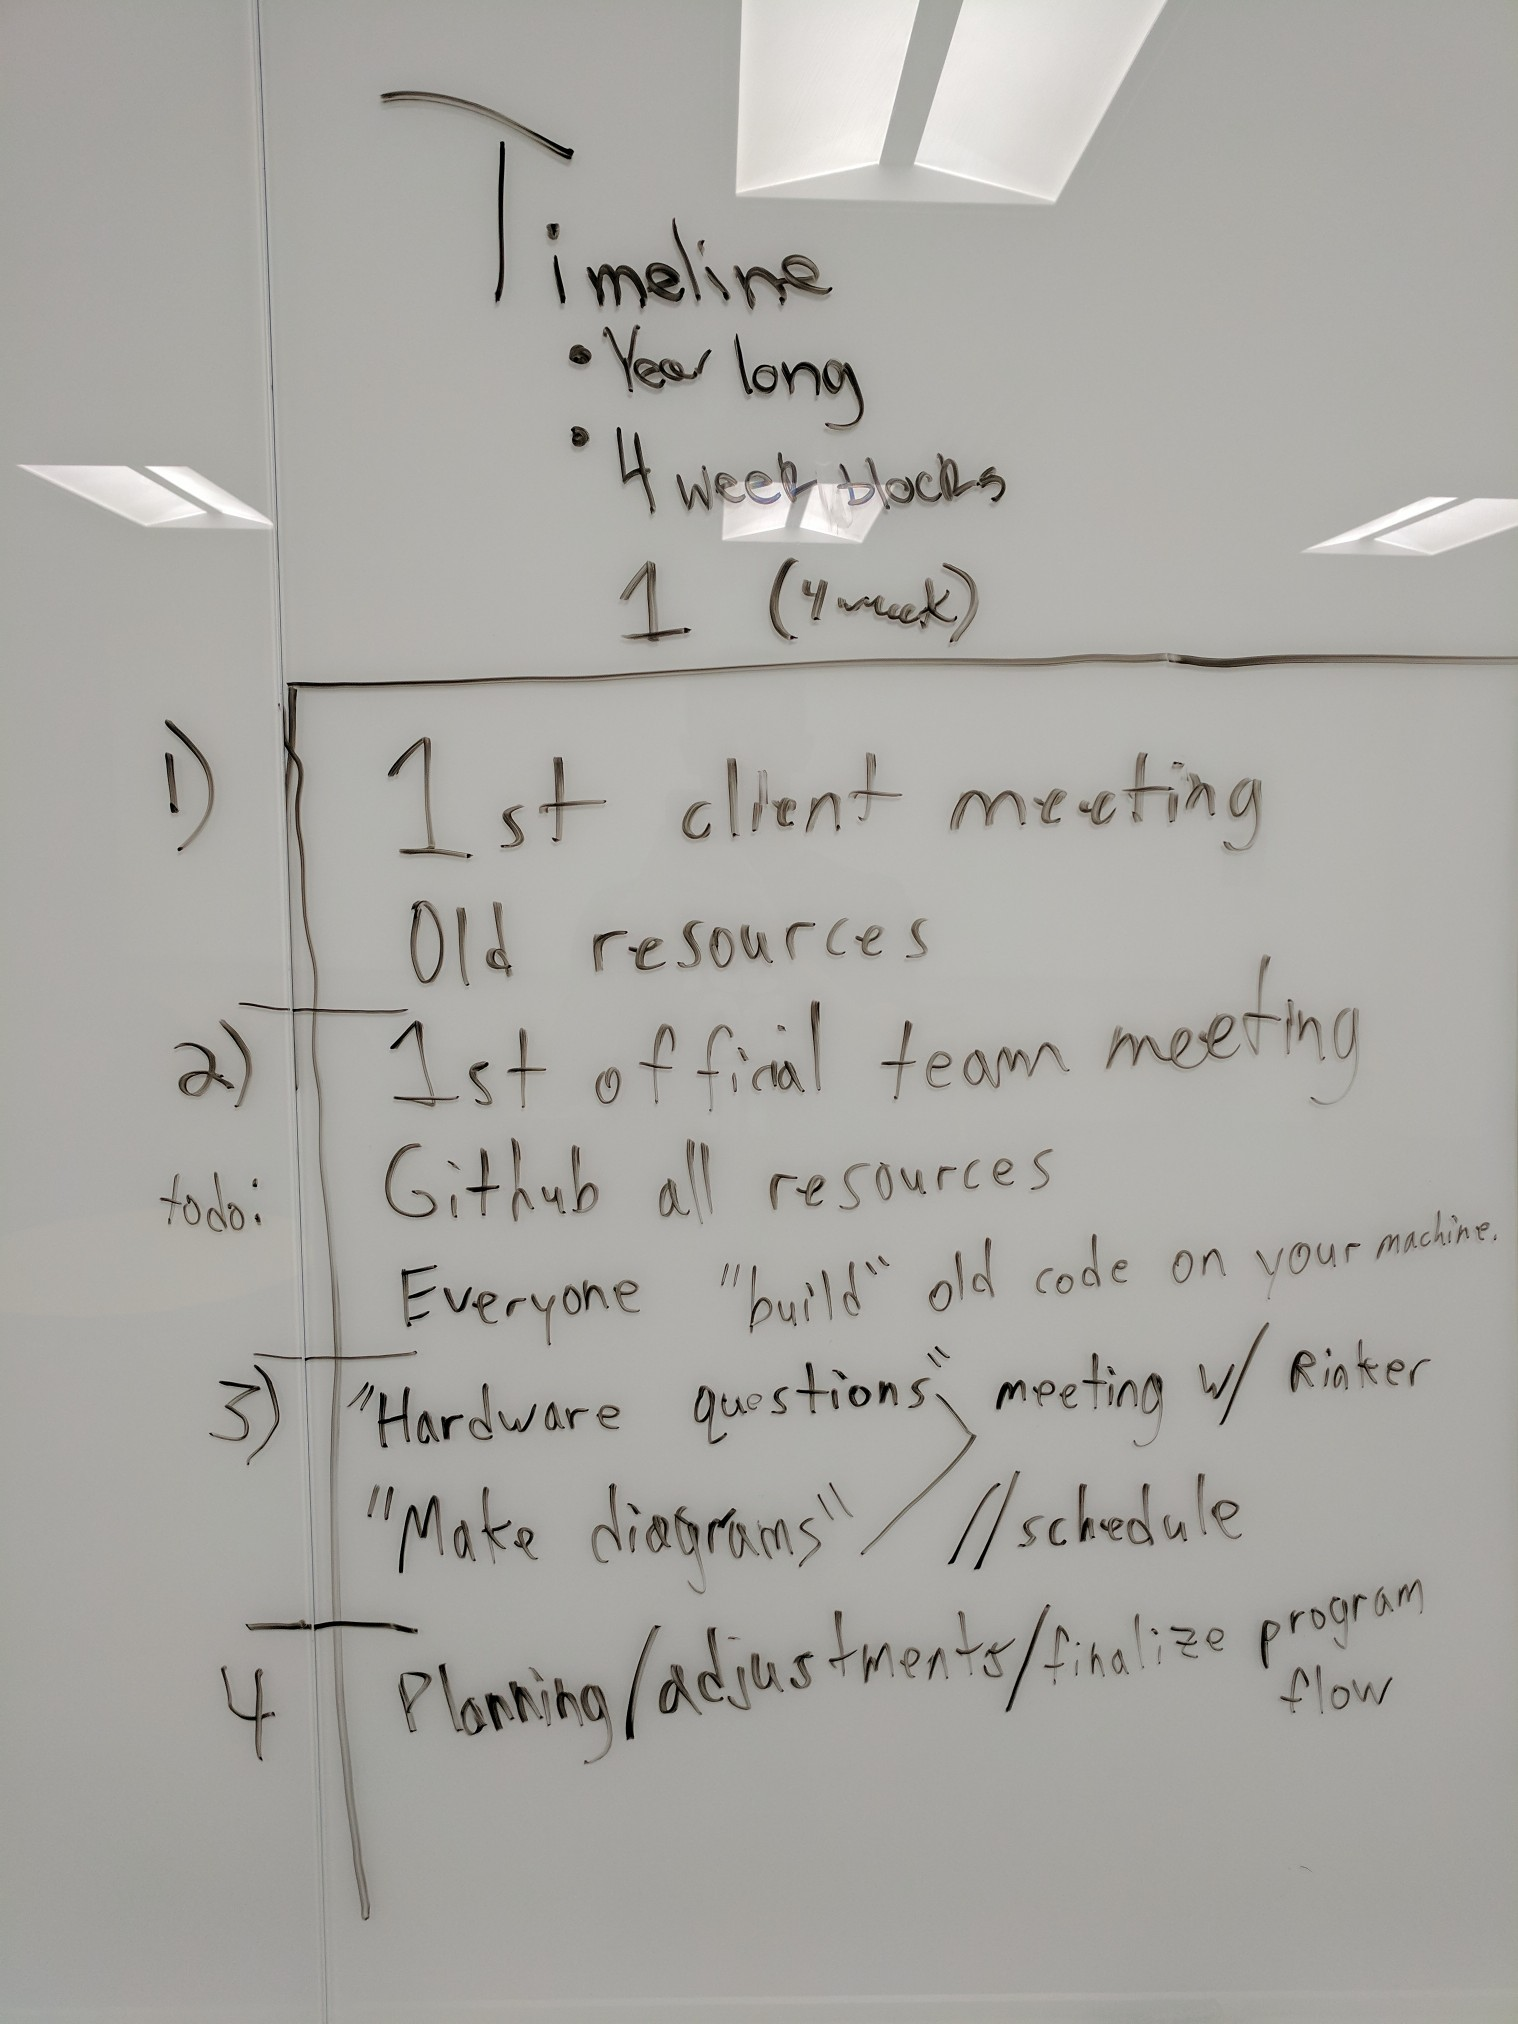
\includegraphics[width=100mm]{9-14_Project_Agenda_1.jpg}
		\caption{9/14 Meeting Project Schedule \label{overflow}}
	\end{figure}

	\begin{figure}[!htb]
		\centering
		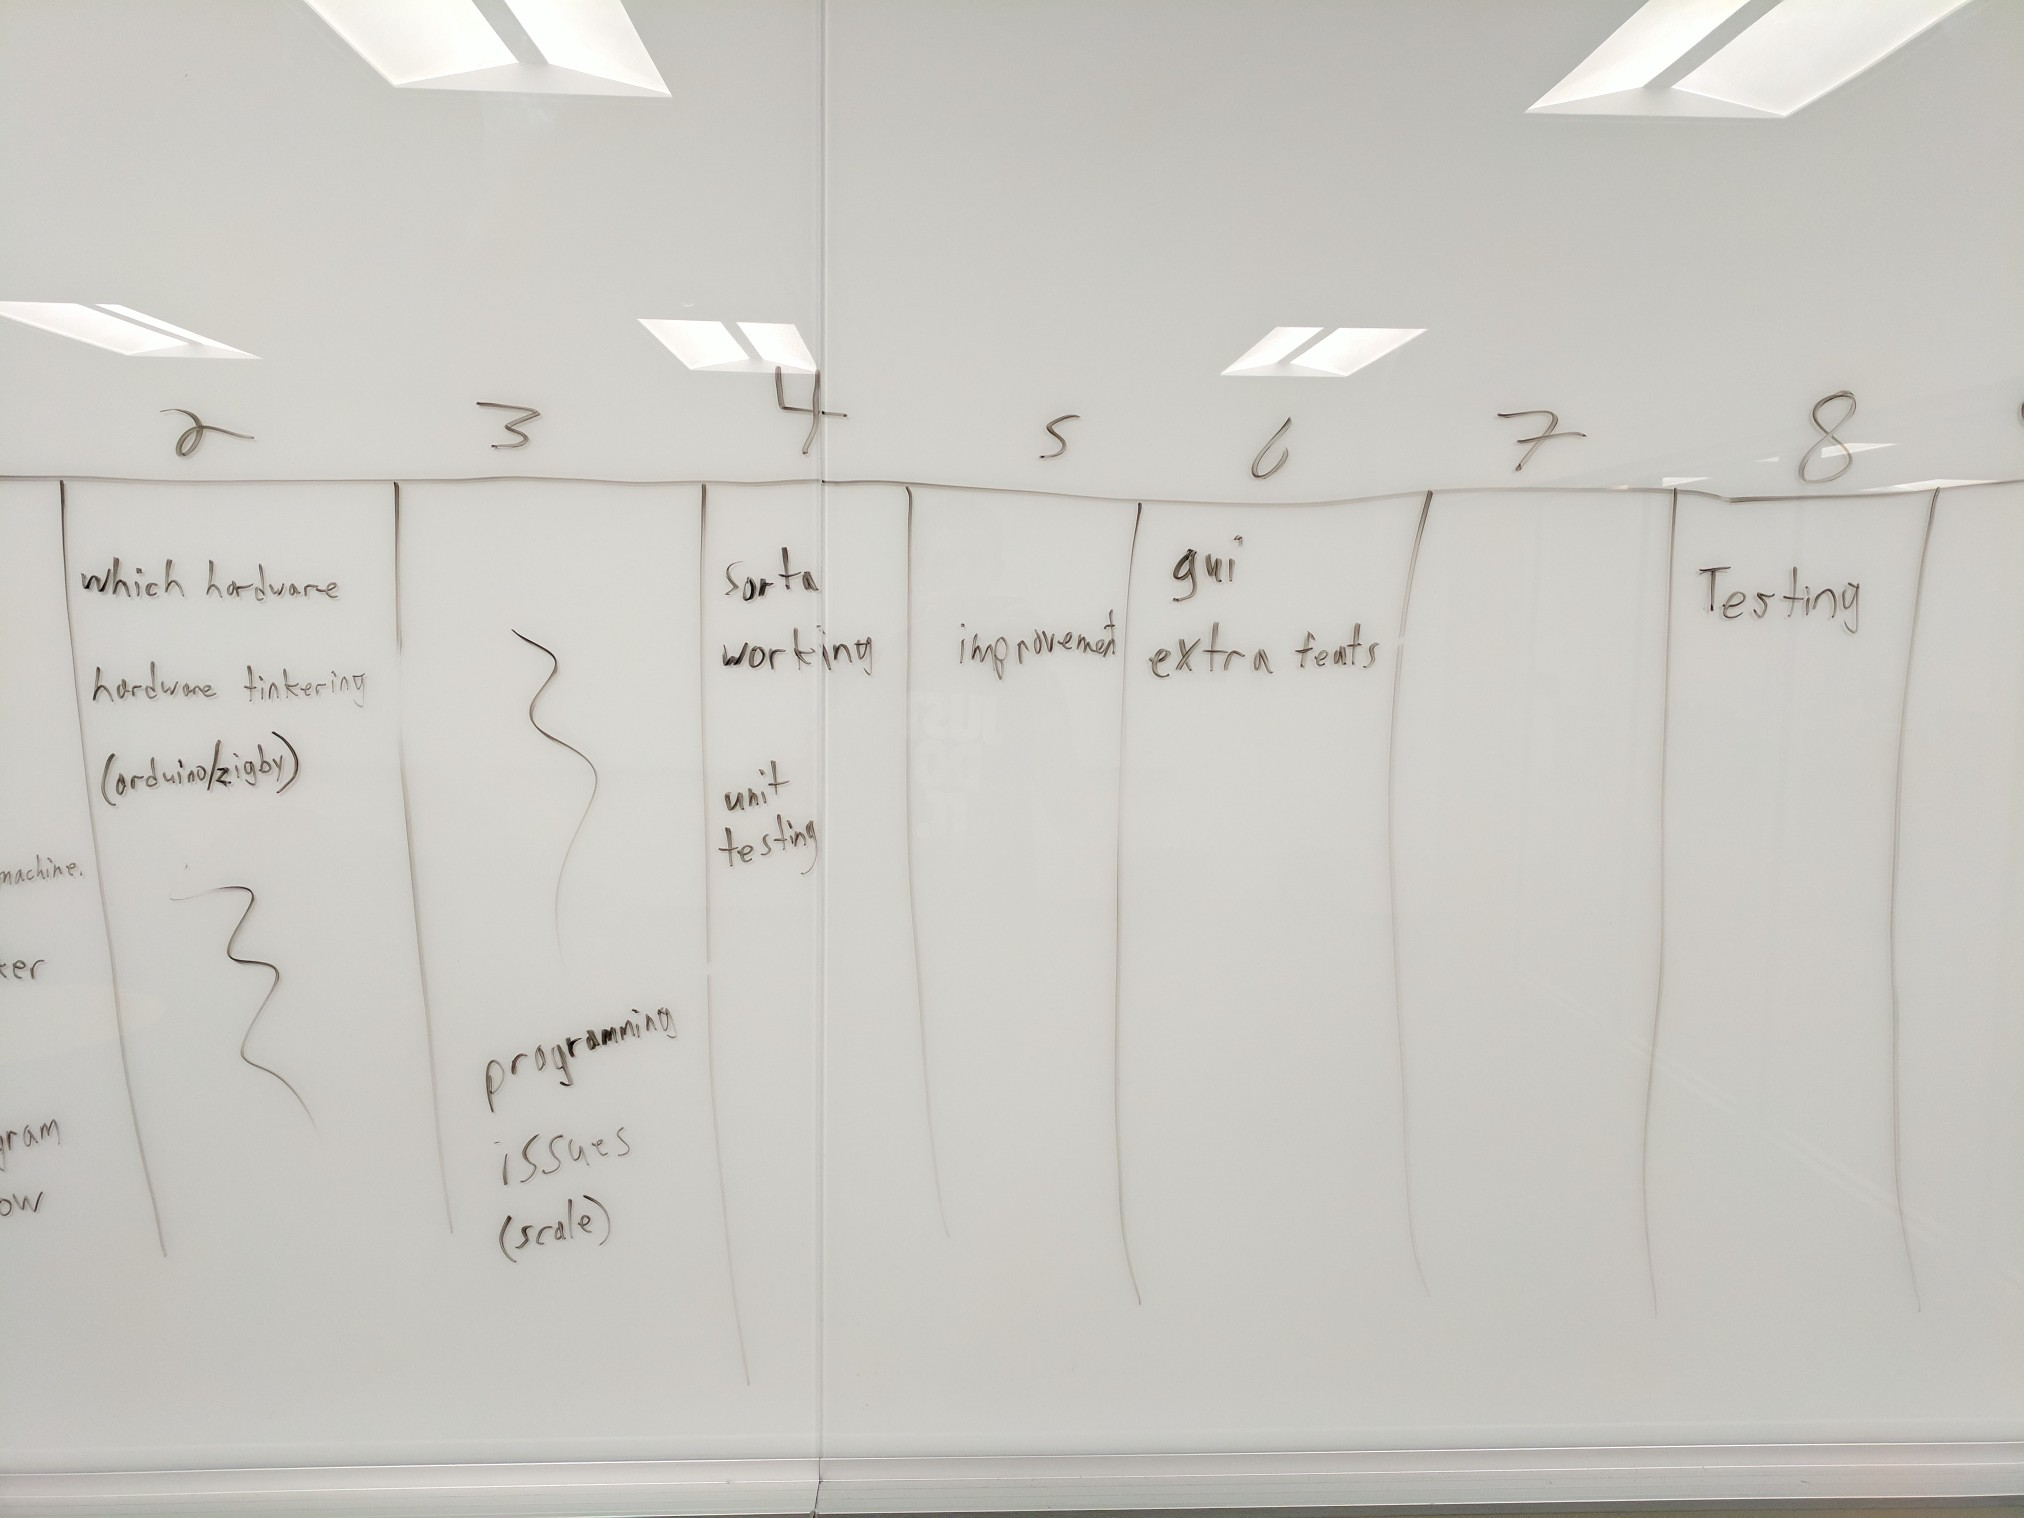
\includegraphics[width=140mm]{9-14_Project_Agenda_2.jpg}
		\caption{9/14 Meeting Project Schedule \label{overflow}}
	\end{figure}
	
	\clearpage
	\subsubsection{9/22/2017 Meeting Notes - With Dr.Rinker}
	All members present, Adrian via Zoom, meeting started at 3:32

We only need to deal with .tan file to hardware, there’s another group redesigning the .tan file creator. They’re finishing up in December. Also may be redesigning the interface for the player?

Current implementation uses xbee to transmit to receiver, then transmits to the light controller serially. 

We can probably use old CSAC space to store hardware, work. This has a soldering station too, along with some goofy glasses and the old tower hardware being stored. 

328p chips are super cheap, could definitely use one of those for each light bar. 

Arduino IDE supports turning off bootloader now, etc, which should make development even easier. 

Current player is Linux specific, supposedly has Mac and Windows equivalent libraries though. Pulseaudio and FTDI. Look into making this cross platform compatible.

Main thread of player sends wav bytes to the audio thread, updates lights once the program reaches the proper time. 

Parts needed: transmitter, shield, USB to serial, receiver chips, light bars themselves, batteries. 

Meeting adjourned at 4:33
	
	% Create new Page (NEED TO USE clearpage because we have pictures that will affect it!)
	\clearpage

\section{Project Learning}
	Technologies used to solve problems are described below. Further discussion of these technologies are left in each section's subsections.

	\newpage
  
\section{Design Goals}
	Client needs and project goals are discussed below. A Timeline for these is also included. Discussion of revision of goals, and addition of any new goals is also discussed below.
	
	\subsection{Client Needs}
	The needs of the Client (University of Idaho) are as follows:
		
		\begin{itemize}
			\item LED Light Bars
			\item Microprocessor communication (Arduino)
			\item LEDs bright enough to be a coherent display, visible from a distance in the dark
			\item Wireless Protocol SPI
			\item Battery powered
			\item Receiver Module for Arduino (802.15.14 chip) 
			\item AdrProcessor for designing chip
			\item Low power mode (sleep mode)
			\item Wake up remotely
			\item 1-bit for each color for each window
			\item 802.15.4 protocol, channels 3 bytes (1 for each color, RGB)
			\item Avoid wifi (we don't want to have interference)
			\item Design module
			\item Expand channels (for expanding bandwidth)
			\item 15-20 stories, need to support enough windows
			\item WAV file support
			\item OSX, Windows, and Linux support (Cross-Platform)
			\item .tan file support - 
		\end{itemize}
	
	\subsection{Project Goal}
	The goal of the project is to the extend the versatility of the Tower Of Lights project, which at the moment, gives the user the ability to run a program which reads in a .tan file (animation files for the lights) and .wav files. Then this
	program communicates with a Arduino via Ethernet. Now, the Arduino communicates to each of the LEDs, and tells them which
	color and brightness to be, from the .tan file (thus it basically reads in animation info). 
	The enhancement of the project involves providing cross-platform support, which means having to rework some of the TowerPlayer code so it doesn't use the Pulse library (which is Linux-specific). Also, the enhancement requires making the wired connection to the Arduinos on the LED bar to wireless, this is accomplished by having an Arduino Receiver on each LED Board that receives info sent out from the Arduino connected to the main computer running the program, that Arduino has a XBee Shield attached, which is a wireless module to transmit the info to each Arduino on a board. The Arduino now requires a portable power supply, which needs to be a 9V battery for each Arduino on an LED Board. The final enhancement is that since the LED Boards are running off battery, they require some kind of sleep mode, where they will still be able to receive info (so they can wake up).\\
	
	The product will give the user the ability to run a program that reads in .tan files and .wav files, have this program communicate with a XBee Wireless module on an Arduino that is attached to a Computer via USB, then communicate wirelessly with each battery powered Arduino receiver, on each LED board, that will then communicate with each LED on that board through wired communication from the Arduino (same one that holds the receiver)to the LEDs. The program that runs through this procedure will be available for the OSX, Windows, and Linux based operating systems.

	\subsection{Timeline}
	This was the timeline for UIdaho's Fall 2017 - Spring 2018 CS 480/481: Senior Capstone Design class.\\
	{ \setstretch{2.0}		
		\scalebox{1}{  		
			\begin{tabular}{r |@{\tline} l}  			
				September  & Planning/Adjustments/Finalize Program Flow 1          \\			
				October & Hardware Decision/Hardware Tinkering (Arduino/Xbee)            \\			
				November & Programming Issues (Scale)\\			
				December & Prototype Product/Unit Testing     \\			
				January & Product Improvement/Evaluation               \\			
				February & GUI Implementation/Extra Features 2          \\			
				March  & TBD                       \\			
				April  & Testing       \\			
				May & Ship/Manufacture (Deliver product)         \\			
			\end{tabular}  		
		}  	
	}
	
	\newpage
    
\section{Specifications and Constraints}
	Discussion of client interviews, pictures, measurements, etc. are provided below. Design specifications and constraints are also presented. Reasoning for any constraints is also mentioned.
	
	\newpage

\section{System Diagrams}
	Discussion of symbols used, the diagrams themselves, and the software used for the diagrams is discussed below.
	
	\subsubsection{Current Product}
	The current product flow in regards to the final product is shown below in Figure below. The current setup does not have any battery setup, and requires a wired connection. Changing this is the core of this project, which will improve the versatility of the TowerOfLights product.
	
		\begin{figure}[ht!]
			\centering
			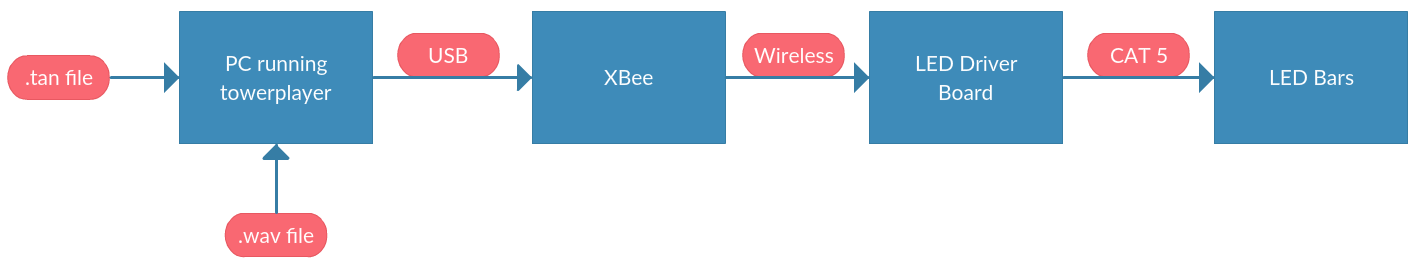
\includegraphics[width=170mm]{What_We_Have.png}
			\caption{Current Product Flow \label{overflow}}
		\end{figure}
	
	
	\subsubsection{Desired Product}
	The desired product flow is shown in the figure below. The main focus is on the battery that should power each Arduino reciever, as well as the SPI protocol from XBee to the Receiver. This is to make the process wireless instead of wired, which is the main goal of this endeavor.
	
	\begin{figure}[ht!]
		\centering
		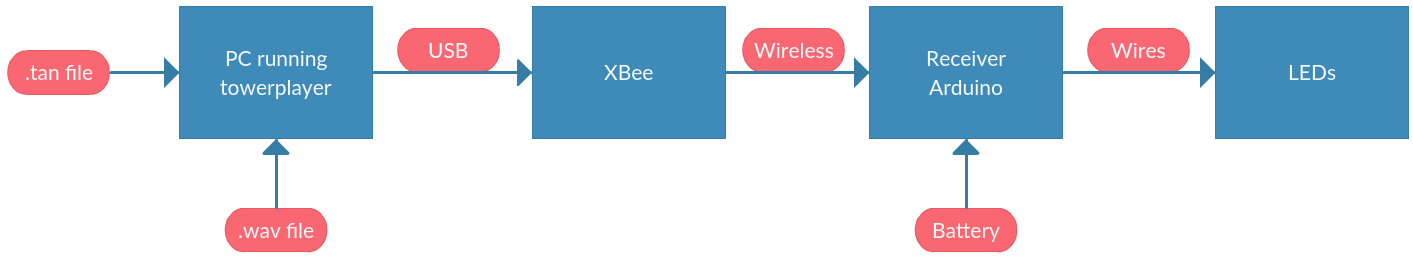
\includegraphics[width=170mm]{What_We_Want.png}
		\caption{Desired Product Flow \label{overflow}}
	\end{figure}


	\subsubsection{PC Running TowerPlayer}
	The diagram for a flow chart depicting the sequence of actions for running the TowerPlayer program on a computer is shown in the figure below. This diagram helps with understanding the underlying software that needs to be setup and used before the hardware can successfully work together.
	
		\begin{figure}[ht!]
			\centering
			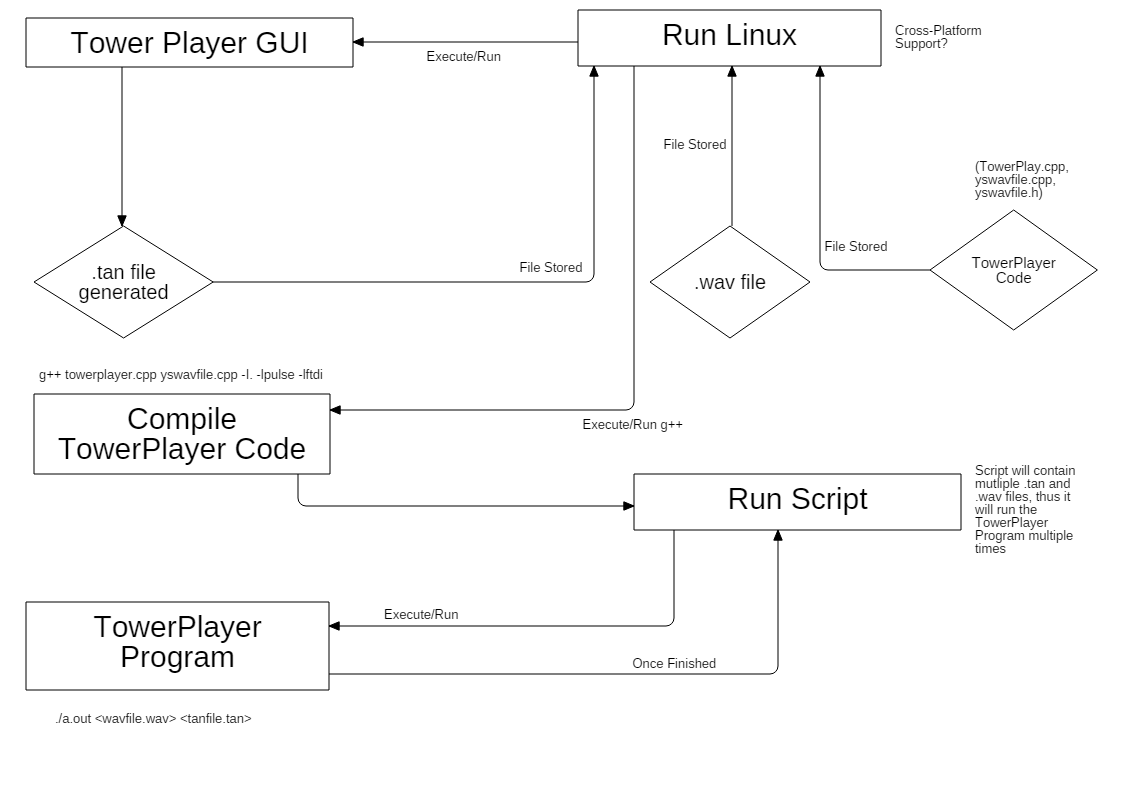
\includegraphics[width=170mm]{PCRunningTowerPlayerFlowChartDiagram.png}
			\caption{Flow Chart Diagram for PC Running TowerPlayer \label{overflow}}
		\end{figure}

	% Create new Page (NEED TO USE clearpage because we have pictures that will affect it!)
	\clearpage

\section{Analysis of Alternatives}
	Discussion of possible alternatives and why some alternatives are better is described below. These topics include: safety, moving parts, cost, durability, compatibility, and reliability.

	\newpage

\section{Engineering Model}
	Discussion of the physical, chemical, and biological system modeling. Also discusses modeling criteria, expected accuracy, and pitfalls. Section of modeling software used is present, as well as data needed and how the data was obtained. Lastly a validation scheme for the model is shown.

	\newpage

\section{Manufacturing/Assembly Plan}
	Discussion of the fabrication need, a flowchart of process oriented projects, a bill of materials, and the estimated manufacturer and delivery time is discussed below.

	\newpage

\section{Experimental Design}
	The characterization of the purpose of the experiment, model validation, data gaps, and performance measurement are discussed below. Also the details on documentation, instrumentation, and measurements are also described.
  	
	\newpage	
  	
\section{Data Analysis}
	Documentation on statistical tools used, accuracy of data, and experiments shown below. Discussion on confidence is results also discussed below.

	\newpage

\section{Balance Sheet}
	Discussion on initial budget, estimated cost for materials, components, labor, and spending plan are all described below.

	\newpage

\section{Other Items}
	File management, archiving, documenting any issues, reports of accidents/incidents/near misses/precautions are described below. 
	
	\subsection{LEaD Design Team Contract}
	The team contract for the \textit{LEaD Design} is shown below. The contract discusses the various professional approaches the team will be held accountable to act towards during the time spent on the project. The contract is an important document, as it dicusses the various inner workings of how the team will work on assignments, resolve conflicts, manage work, make decisions and so on. The contract is four pages total.
	
		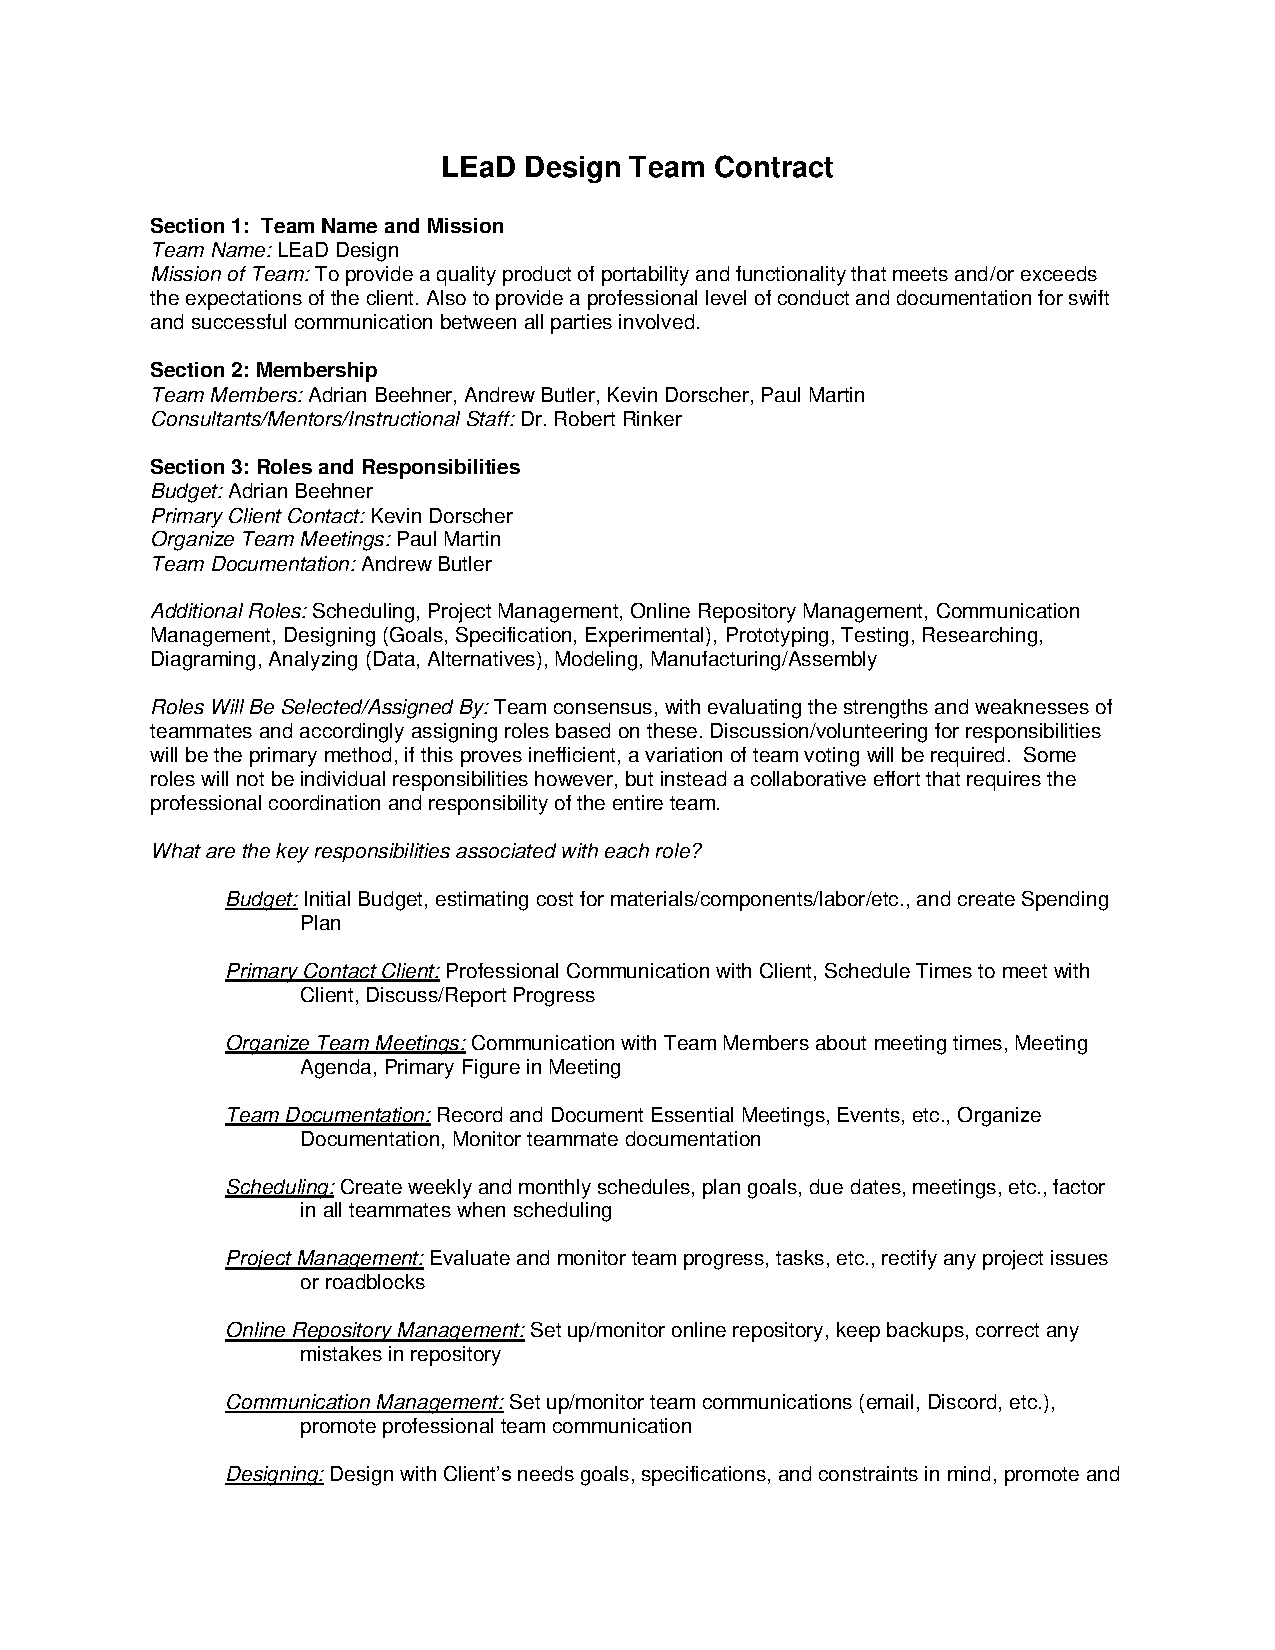
\includepdf[pages={-}, scale =1, pagecommand={}]{LEaD_Design_Team_Contract.pdf}			% {-} means include all pages
		


\end{document}
